\documentclass[11pt]{beamer}
\usepackage[utf8]{inputenc}
\usepackage[T1]{fontenc}
\usepackage[french]{babel}
\usepackage{lmodern}

\usepackage{amsmath}
\usepackage{amsfonts}
\usepackage{amssymb}
\usepackage{stmaryrd}
\usepackage{algorithm}
\usepackage{algorithmic}
\usepackage{hyperref}

\usetheme{default}
\author{Pierre Gimalac et Alexandre Moine}
\begin{document}
\title{Model-checking de Computation Tree Logic}
%\subtitle{}
%\logo{}
%\institute{}
\date{5 juin 2019}
%\subject{}
%\setbeamercovered{transparent}
%\setbeamertemplate{navigation symbols}{}

\begin{frame}[plain]
	\maketitle
\end{frame}

\section*{Plan}

\begin{frame}
	\frametitle{Plan}
	\tableofcontents[]
\end{frame}

\section{CTL}
\subsection{Structure de Kripke}
\begin{frame}
    \frametitle{CTL}
    \framesubtitle{Structure de Kripke}

    $(Q,T, q_0, l)$:
    \begin{itemize}
    \item $Q$ est un ensemble d'états
    \item $T \subseteq Q \times Q$ est une relation de transition
    \item $q_0 \in Q$ est l'état de départ
    \item $l : Q \to \mathcal{P}(\Omega)$ est une fonction d'étiquetage
    \end{itemize}

    \pause
    \bigskip
    \textit{On considère le cas où $Q$ est fini et $T$ vérifie que tout élément est en relation avec au moins un élément}\\
    \pause
    \bigskip
    Une exécution de $\mathcal{A} = (Q, T, q_0, l)$ est une fonction $\sigma : \mathbb{N} \to Q$ telle que $(\sigma(i), \sigma(i+1))\in T$. $Exec_\mathcal{A}(q)$ est l'ensemble des exécutions $\sigma$ de $\mathcal{A}$ telles que $\sigma(0) = q$.
\end{frame}

\subsection{Grammaire}
\begin{frame}
	\frametitle{Computation Tree Logic}
    \framesubtitle{Grammaire}

    \begin{align*}
    \phi &::= \bot \mid \top \mid p \mid \neg \phi \mid \phi\land\phi \mid \phi\lor\phi \mid \\
    &\quad \mbox{AX }\phi \mid \mbox{EX }\phi \mid
    \mbox{A }\phi \mbox{ W } \phi \mid \mbox{E }\phi \mbox{ W } \phi \mid
    \mbox{A }\phi \mbox{ U } \phi \mid \mbox{E }\phi \mbox{ U } \phi
    \end{align*}

    \pause
    \small
    On définit aussi:
    \begin{itemize}
        \item $\mbox{EF } \phi := \mbox{E } \top \mbox{ U } \phi$
        \item $\mbox{AF } \phi := \mbox{A } \top \mbox{ U } \phi$
        \item $\mbox{EG } \phi := \neg (\mbox{AF } (\neg \phi))$
        \item $\mbox{AG } \phi := \neg (\mbox{EF } (\neg \phi))$
    \end{itemize}
\end{frame}

\subsection{Sémantique}
\begin{frame}
    \frametitle{Computation Tree Logic}
    \framesubtitle{Sémantique}

    \footnotesize
    \begin{tabular}{lcl}
    $q \vDash \top$ && est toujours vrai\\
    $q \vDash \bot$ && n'est jamais vrai\\
    $q \vDash p$ &ssi&
    $p \in l (q)$\\
    \pause[2]&& $p$ est une étiquette de $q$\pause[1]\\
    $q \vDash \neg \psi$ &ssi&
    $q \nvDash \psi$\\
    \pause[2]&& $q$ ne vérifie pas $\psi$\pause[1]\\

    $q \vDash \psi_1 \land \psi_2$ &ssi&
    $q \vDash \psi_1\land q \vDash \psi_2$\\
    \pause[2]&& $q$ vérifie $\phi_1$ et $q$ vérifie $\phi_2$\pause[1]\\

    $q \vDash \psi_1 \lor \psi_2$ &ssi&
    $q \vDash \psi_1\lor q \vDash \psi_2$\\
    \pause[2]&& $q$ vérifie $\phi_1$ ou $q$ vérifie $\phi_2$\pause[1]\\

    $q \vDash \mbox{EX } \psi$ &ssi&
    $\exists \sigma \in Exec_\mathcal{A}(q)$, $\sigma(1) \vDash \psi$\\
    \pause[2]&& il existe un successeur de $q$ vérifiant $\psi$\pause[1]\\

    $q \vDash \mbox{AX } \psi$ &ssi&
    $\forall \sigma \in Exec_\mathcal{A}(q)$, $\sigma(1) \vDash \psi$\\
    \pause[2]&& tous les successeurs de $q$ vérifient $\psi$\pause[1]\\

    \end{tabular}
\end{frame}

\begin{frame}
    \frametitle{Computation Tree Logic}
    \framesubtitle{Satisfaction}

    \footnotesize
    \begin{tabular}{lcl}
    $q \vDash \mbox{E } \psi_1 \mbox{ U } \psi_2$ &ssi&
    $\exists \sigma \in Exec_\mathcal{A}(q)$, $\exists k \in \mathbb{N}$,\\
    &&$\sigma(k)\vDash \psi_2$ $\land$ $\forall j \in \llbracket 0; k\llbracket, \sigma(j)\vDash \psi_1$\\
    && \pause[2] il existe un chemin à partir de $q$ tel que $\psi_1$\\&& est vrai jusqu'à ce que $\psi_2$ le soit (et il le sera un jour) \pause[1]\\

    $q \vDash \mbox{A } \psi_1 \mbox{ U } \psi_2$ &ssi&
    $\forall \sigma \in Exec_\mathcal{A}(q)$, $\exists k \in \mathbb{N}$,\\
    &&$\sigma(k)\vDash \psi_2$ $\land$ $\forall j \in \llbracket 0; k\llbracket, \sigma(j)\vDash \psi_1$\\
    &&\pause[2] pour tout chemin partant de $q$, $\psi_1$ est vrai \\&& jusqu'à ce que $\psi_2$ le soit (et il le sera un jour)\pause[1]\\

    $q \vDash \mbox{E } \psi_1 \mbox{ W } \psi_2$ &ssi&
    $\exists \sigma \in Exec_\mathcal{A}(q)$, soit $\forall j \in \mathbb{N}$, $\sigma(j) \vDash \psi_1$\\
    & & \pause[2]soit $\exists k\in \mathbb{N}$: $\sigma(k)\vDash \psi_2 \land \forall j \in \llbracket i; k \llbracket$: $\sigma(j) \vDash \psi_1$\\
    && il existe un chemin à partir de $q$ tel que $\psi_1$\\&& est vrai jusqu'à ce que, peut-être, $\psi_2$ le soit\pause[1]\\

    $q \vDash \mbox{A } \psi_1 \mbox{ W } \psi_2$ &ssi&
    $\forall \sigma \in Exec_\mathcal{A}(q)$, soit $\forall j \in \mathbb{N}$, $\sigma(j) \vDash \psi_1$\\
    & & \pause[2]soit $\exists k\in \mathbb{N}$: $\sigma(k)\vDash \psi_2 \land \forall j \in \llbracket i; k \llbracket$: $\sigma(j) \vDash \psi_1$\\
    && pour tout chemin partant de $q$, $\psi_1$ est vrai \\&& jusqu'à ce que, peut-être, $\psi_2$ le soit\pause[1]\\
    \end{tabular}

\end{frame}


\section{Model-checking par résolution de jeu faible de parité}
\subsection{Jeu de parité}
\begin{frame}
	\frametitle{Model-checking par résolution de jeu faible de parité}
    \framesubtitle{Jeu de parité}

    $(V_E, V_A, R, c)$:
    \begin{itemize}
        \item $V_E$ (respectivement $V_A$) est l'ensemble des états jouables par Ève (respectivement Adam). On demande de plus que $V_E \cap V_A = \emptyset$. On note $V = V_E \sqcup V_A$.
        \item $R \subseteq V \times V$ est une relation de transition.
        \item $c : V \to (\mathbb{N} \cup \{\bot\})$ est une fonction qui associe une couleur ou $\bot$ à chaque état.
    \end{itemize}
\end{frame}

\subsection{Partie, victoire et stratégie}
\begin{frame}
    \frametitle{Model-checking par résolution de jeu faible de parité}
    \framesubtitle{Partie, victoire et stratégie}

    Une partie est une fonction $\omega : V' \to V, V' \subseteq V$ telle que $\forall v \in V', (v,\omega(v)) \in R$

    \pause
    \bigskip

    Une partie est gagnée par Ève à partir d'un état $q_0 \in V$ si est seulement si:
    \begin{itemize}
    \item Soit Adam est bloqué : $\exists n \in \mathbb{N}, \omega^n (q_0) \in V_A\backslash V'$.
    \item Soit le minimum des couleurs (des états par lesquels on passe) que l'on voit une infinité de fois est pair.
    \end{itemize}

    \pause
    \bigskip

    On appelle une stratégie pour Ève (respectivement Adam) une fonction $\rho : V_E' \to V$ (respectivement $\rho : V_A' \to V$), $V_E' \subseteq V_E$ et $V_A' \subseteq V_A$, telle que pour chaque $v$ dans $V_E'$ (respectivement $V_A'$), $(v, \rho(v)) \in R$.
\end{frame}

\subsection{Jeu faible de parité}
\begin{frame}
    \frametitle{Model-checking par résolution de jeu faible de parité}
    \framesubtitle{Jeu faible de parité}

    On dit qu'un jeu de parité $G = (V_E,V_A,R,c)$ est \emph{faible}  si et seulement s'il existe $V_1$, ..., $V_k$ une partition de $V = V_E \sqcup V_A$ telle que:
    \begin{enumerate}[a)]
    \item La couleur soit la même pour tous les états d'une classe de la partition : $\forall i \in \llbracket 1 ; k \rrbracket$, $\forall x, y \in V_i$, $(c(x) \neq \bot \land c(y) \neq \bot)  \implies c(x) = c(y)$.
    \item La partition représente une convergence du jeu :\\
    $\forall (x, y) \in R$, $x\in V_i, y \in V_j \Rightarrow i \leq j$.
    \end{enumerate}
\end{frame}


\subsection{Algorithme}
\footnotesize
\begin{algorithm}[h!]
    \caption{$solve\_weak\_game$}
\begin{algorithmic}[1]
    \REQUIRE $(q_0, V, E)$ \COMMENT{l'état de départ et le graphe du jeu}
    \STATE $CFC \leftarrow compute\_cfc(V, E)$
    \STATE $CFC \leftarrow topological\_sort(CFC)$
    \STATE $CFC \leftarrow reverse(CFC)$
    \STATE $winners \leftarrow new\_array(size(V), \bot)$
    \FOR { $V_k \in CFC$ }
        \STATE $\gamma \leftarrow get\_winner(V_k)$
        \STATE $propagate\_opposite(\gamma, V_k, E, winners)$
        \FOR { $x \in V_k$ }
            \IF { $winners[x] = \bot$ }
                \STATE $winners[x] = \gamma$
            \ENDIF
        \ENDFOR
    \ENDFOR
    \RETURN $winners[q_0]$
\end{algorithmic}
\end{algorithm}

\begin{algorithm}[h!]
\caption{$propagate\_opposite$}

\begin{algorithmic}[1]
    \scriptsize
    \REQUIRE $(\gamma, V, E, winners)$
    \STATE $CHANGED \leftarrow FALSE$
    \FOR{$x \in V$}
        \IF{$winners[x] = \bot$}
            \STATE $EXI \leftarrow FALSE$
            \STATE $ALL \leftarrow TRUE$
            \FOR {$(x,y) \in E$}
                \IF{$winners[y] = \overline{\gamma}$}
                    \STATE $EXI \leftarrow TRUE$
                \ELSE
                    \STATE $ALL \leftarrow FALSE$
                \ENDIF
            \ENDFOR
            \IF{$(get\_player(x) = \overline{\gamma} \land EXI) \lor ALL $}
                \STATE $CHANGED \leftarrow TRUE$
                \STATE $winners[x] = \overline{\gamma}$
                \STATE BREAK \COMMENT{Non nécessaire, mais simplifie la preuve}
            \ENDIF
        \ENDIF
    \ENDFOR
    \IF{$CHANGED$}
        \STATE $propagate\_opposite(\gamma, V, E, winners)$
    \ENDIF
    \RETURN
\end{algorithmic}
\end{algorithm}

\subsection{Plan de preuve de correction}
\begin{frame}
	\frametitle{Plan de preuve de correction}
	$solve\_weak\_game$ termine. \\
	\bigskip \pause
	$solve\_weak\_game$ est correct: par récurrence sur les CFC (ordonnées par ordre topologique inversé), on montre qu'après traitement, $winners[x]$ contient le gagnant de l'état $x$.
	\begin{itemize}
		\item Pour une "feuille" de l'arbre des CFC $propagate\_opposite$ est correct.
		\item Pour une CFC plus haute dans l'arbre, les états internes ne peuvent que mener à des états d'une CFC plus basse, dont on connait les gagnants par hypothèse de récurrence, ce qui permet de montrer dans $propagate\_opposite$ que:
		\begin{itemize}
			\item $EXI$ est à $TRUE$ $\iff$ il existe un successeur gagnant.
			\item $ALL$ est à $TRUE$ $\iff$ tous les successeurs sont gagnants.
		\end{itemize}
	\end{itemize}
\end{frame}

\section{Model-checking par marquage}
\subsection{Principe}
\begin{frame}
    \frametitle{Model-checking par marquage}
    \framesubtitle{Principe}
    L'algorithme de marquage de la structure de Krikpe $\mathcal{A} = (Q, T, q_0, l)$ pour une formule $\phi$ se fait récursivement avec les sous formules.\\\bigskip

    On renvoie à chaque étape un tableau qui associe à chaque état de $Q$ un booléen.
\end{frame}

\begin{frame}
    \frametitle{Model-checking par marquage}
    \framesubtitle{Algorithme informel}

    Dans une structure de Kripke $\mathcal{A}=(Q, T, q_0, l)$:\\\bigskip
    \begin{tabular}{lcl}
        $marquage(\top)[q] = \top$&&\\
        $marquage(\bot)[q] = \bot$&&\\
        $marquage(p)[q] = \top$&ssi& $p\in l[q]$\\
        $marquage(\neg \phi)[q] = \top$&ssi&$marquage(\phi)[q] = \bot$\\
        $marquage(\phi \lor \psi)[q] = \top$&ssi&$marquage(\phi)[q] = \top \lor marquage(\psi)[q] = \top$\\
        $marquage(\phi \land \psi)[q] = \top$&ssi&$marquage(\phi)[q] = \top \land marquage(\psi)[q] = \top$\\
        $marquage(EX\phi)[q] = \top$&ssi&$\exists (q, q') \in T, marquage(\phi)[q'] = \top$\\
        $marquage(AX\phi)[q] = \top$&ssi&$\forall (q, q') \in T, marquage(\phi)[q'] = \top$\\
    \end{tabular}
\end{frame}

\begin{frame}
    \frametitle{Model-checking par marquage}
    \framesubtitle{Algorithme informel}

\end{frame}

\subsection{Exemple}
\begin{frame}
    \frametitle{Model-checking par marquage}
    \framesubtitle{Exemple: a$\lor$c}

    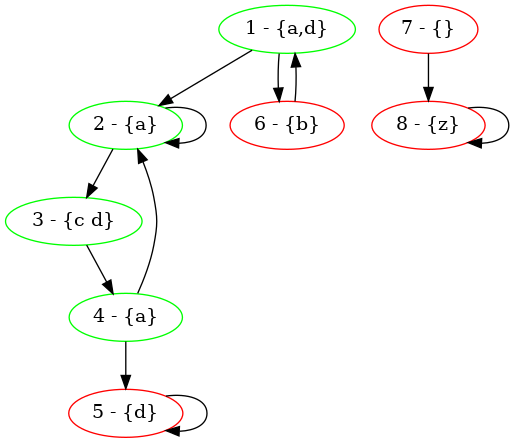
\includegraphics[scale=0.4]{imgs/marquage1.png}
\end{frame}

\begin{frame}
    \frametitle{Model-checking par marquage}
    \framesubtitle{Exemple: b}

    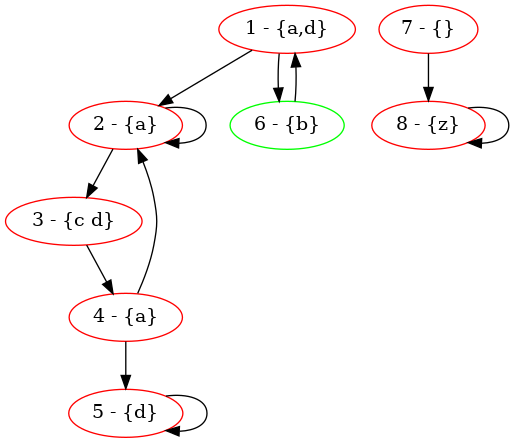
\includegraphics[scale=0.4]{imgs/marquage2.png}
\end{frame}

\begin{frame}
    \frametitle{Model-checking par marquage}
    \framesubtitle{Exemple: E a$\lor$c W b}

    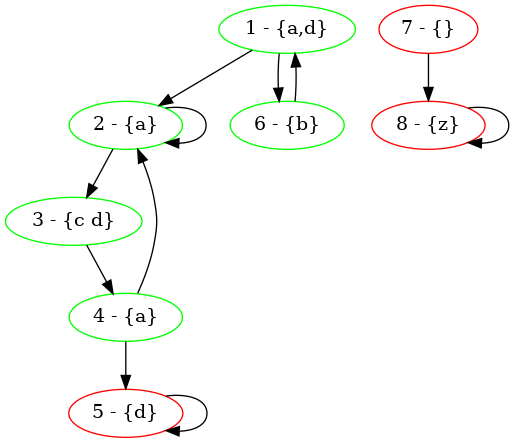
\includegraphics[scale=0.4]{imgs/marquage3.png}
\end{frame}

\begin{frame}
    \frametitle{Model-checking par marquage}
    \framesubtitle{Exemple: AX E a$\lor$c W b}

    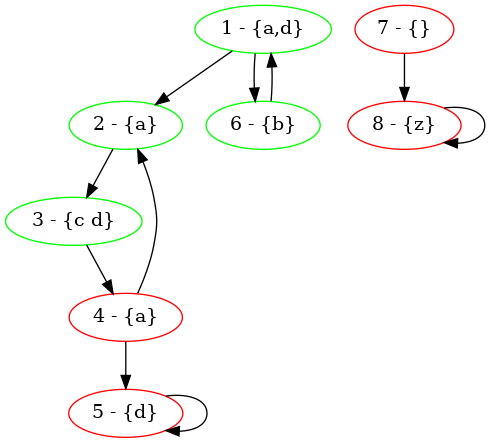
\includegraphics[scale=0.4]{imgs/marquage4.png}
\end{frame}

\section*{Conclusion}
\begin{frame}
    \frametitle{Conclusion}
\end{frame}

\end{document}
